\chapter{Numeri Naturali}
\label{cha:NumeriNaturali}
\minitoc
\mtcskip                                % put some skip here
\minilof                                % a minilof
\mtcskip                                % put some skip here
\minilot
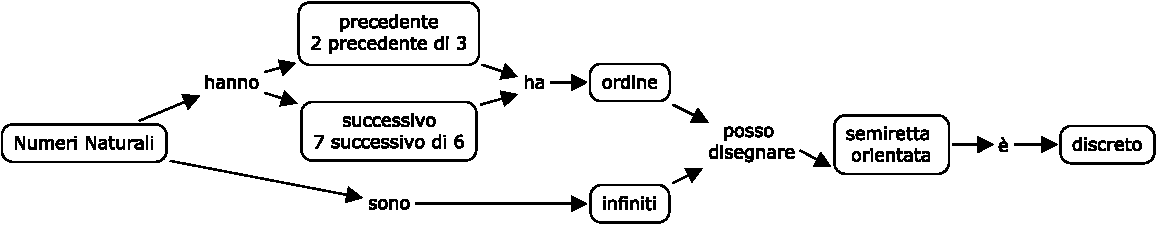
\includegraphics[scale=0.80]{NumeriNaturali-crop}
\section{Addizione}
\label{sec:NumerinatADD}
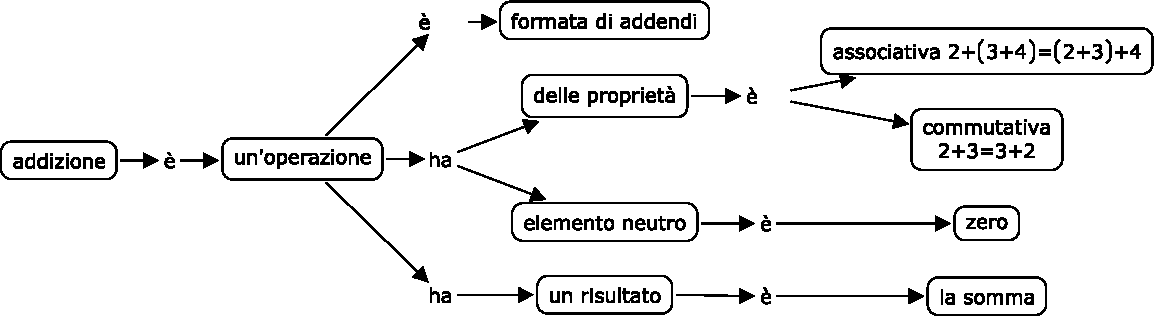
\includegraphics[scale=0.80]{Numerinaturali_somma-crop}
\section{Sottrazione}
\label{sec:NumerinatDiff}
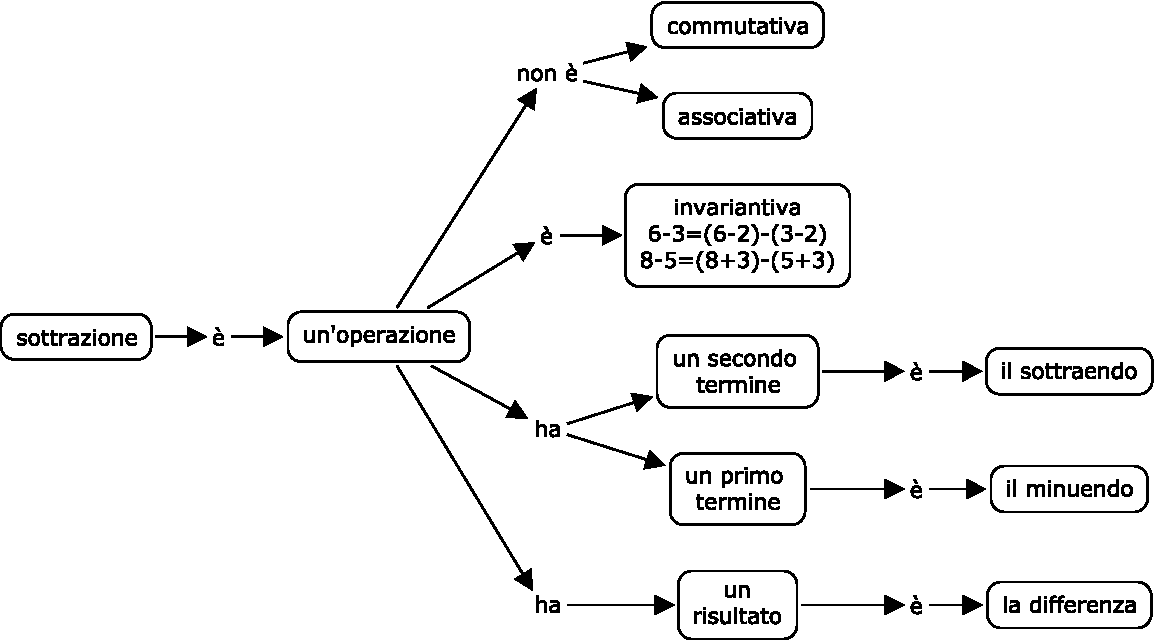
\includegraphics[scale=0.80]{Numerinaturali_differenza-crop}
\section{Moltiplicazione}
\label{sec:NumerinatMolt}
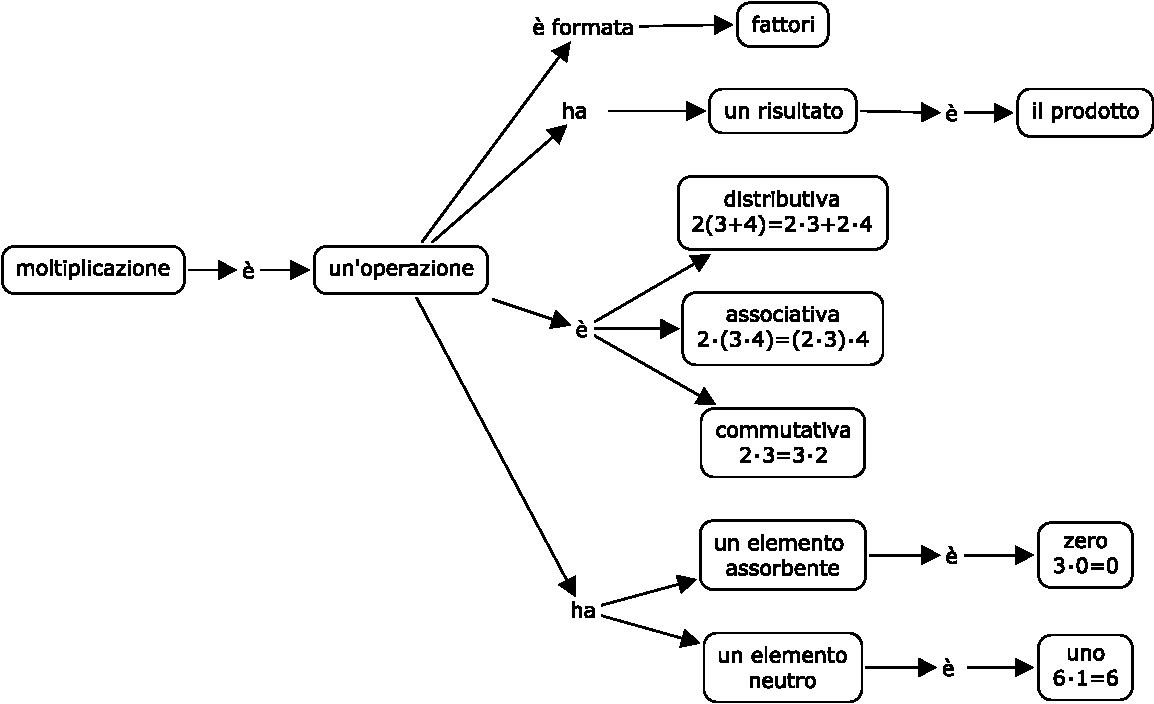
\includegraphics[scale=0.80]{Numerinaturali_prodotto-crop}
\section{Divisione}
\label{sec:Numerinatdiv}
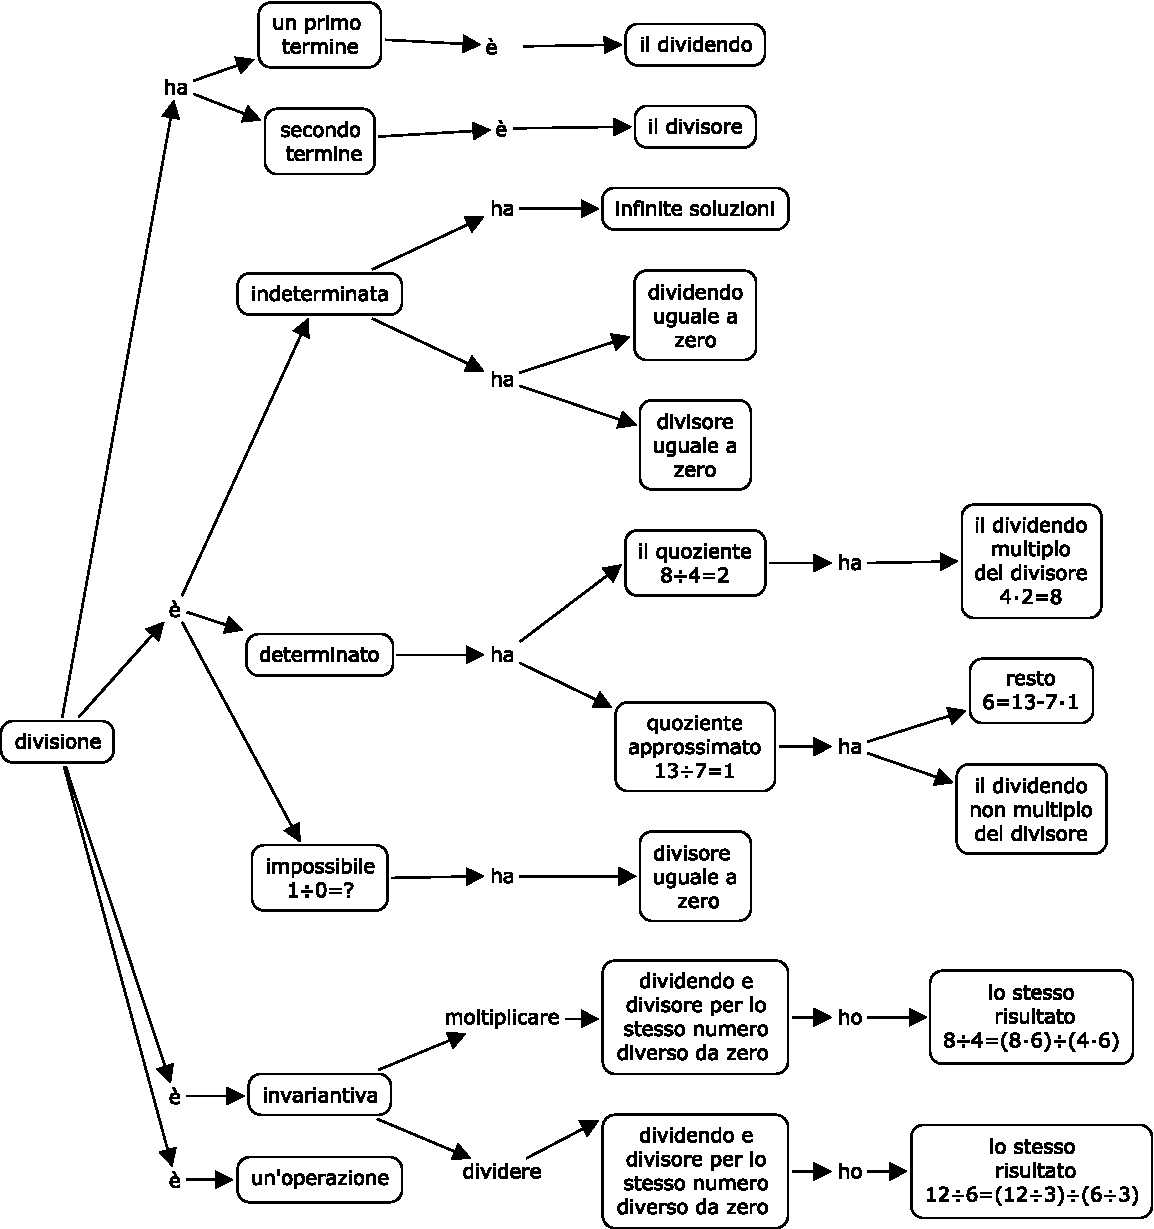
\includegraphics[scale=0.80]{Numerinaturali_divisione-crop}
\section{Potenza}
\label{sec:NumerinatPot}
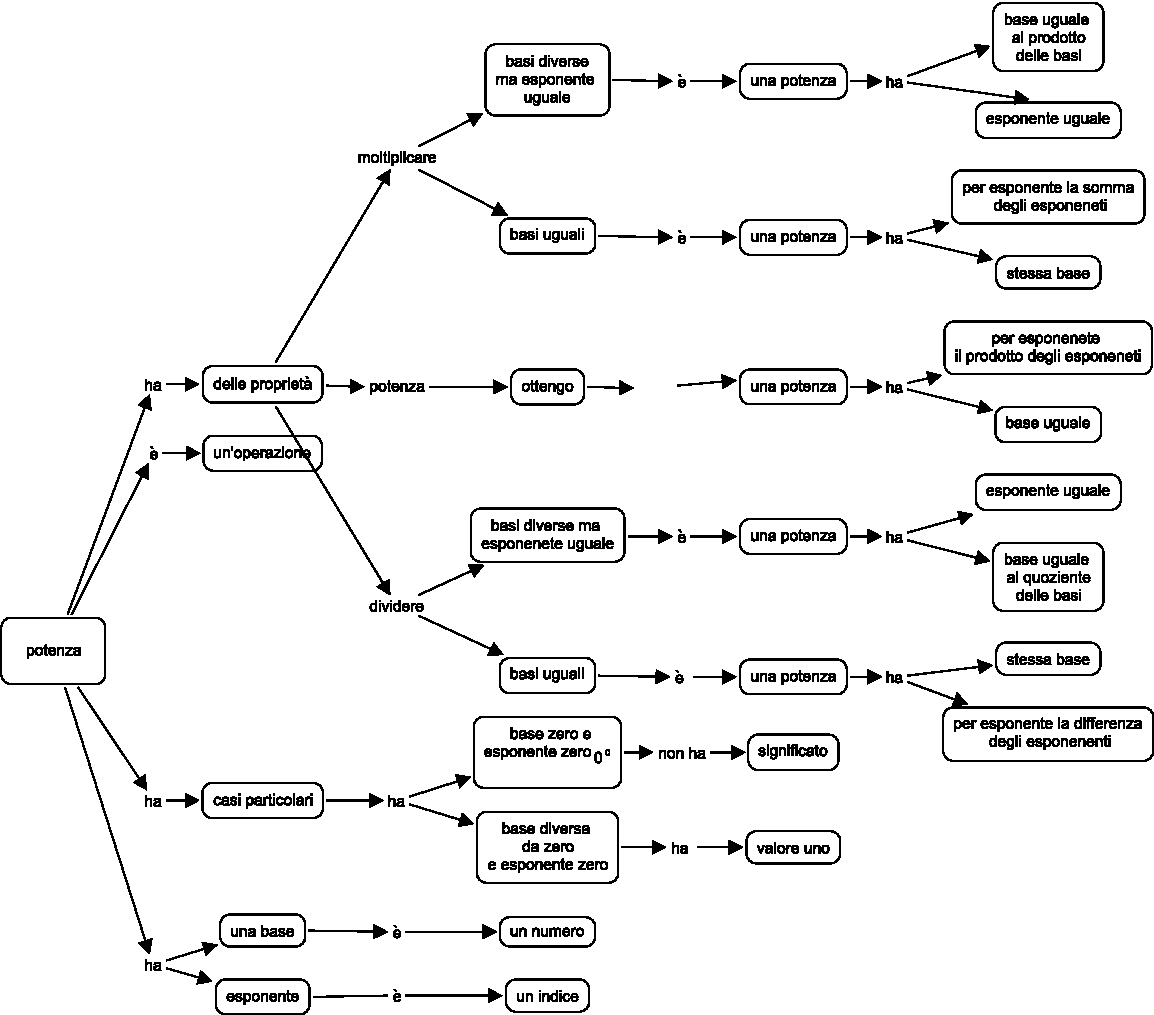
\includegraphics[scale=0.80]{Numerinaturali_potenza-crop}
\section{Numeri primi e composti}
\label{sec:Numeriprimiecomposti}
Una possibile classificazione dei numeri naturali è la seguente
\begin{center}
	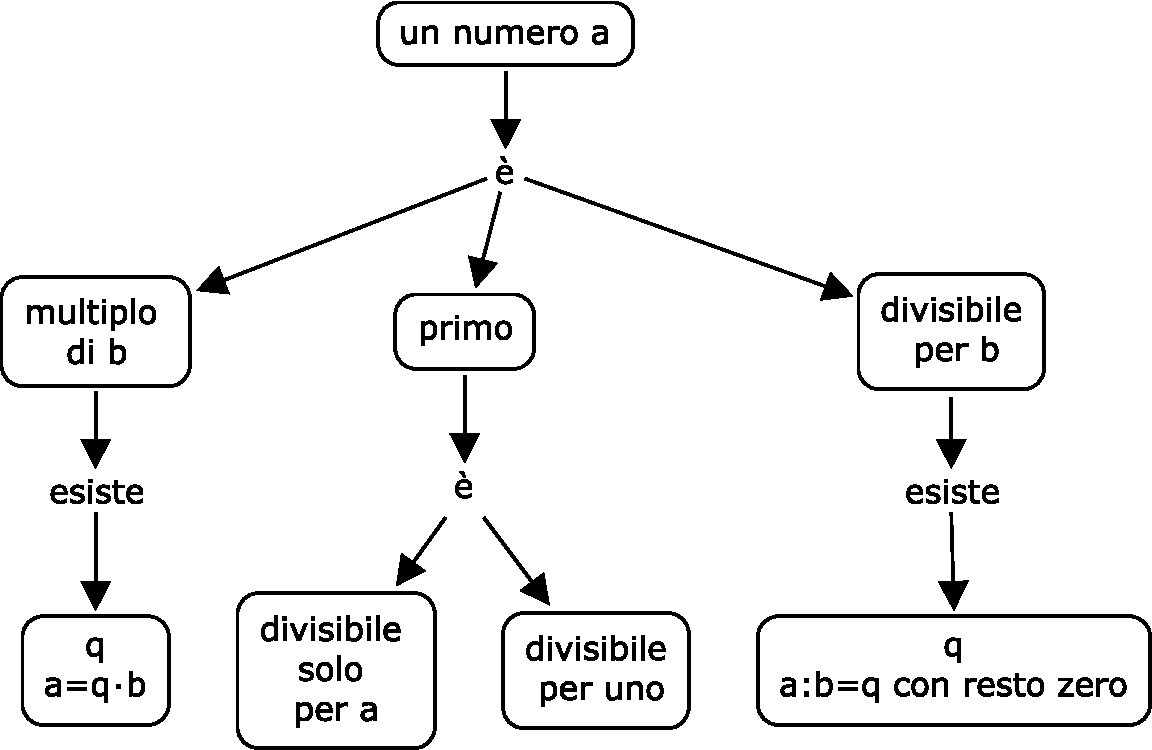
\includegraphics[scale=0.70]{NumeriNaturali_primi-crop}
\end{center}
Quindi, per esempio, dato che $18:2=9$ con resto zero avremo:
\begin{enumerate}
	\item 18 è multiplo di 2 secondo 9
	\item 18 è divisibile per 2
\end{enumerate}
\subsection{Scomposizione in fattori primi}
Per scomporre un numero naturale come prodotto di numeri primi  si può usare  l'algoritmo\nobs\vref{fig:numnatscposizionefattori}
	
\begin{figure}
\centering
\begin{tikzpicture}[auto, -stealth, thick]
% Definizione dei nodi e delle loro scatole
\tikzstyle{line} = [draw,->]
\node[ellipse,draw ]  (primo) {Inizio};
\node[rectangle,draw, text width=6cm,align=flush center, below of=primo, node distance=5em]  (secondo) {dividi il numero dato per
	il più piccolo primo che lo divide};
\node[diamond,draw, below of=secondo,node distance=10em]  (terzo) {il quoziente è uno?};
\node[ellipse, draw,below of=terzo,node distance=10em ] (quarto) {Fine};

% collegamento dei nodi
\begin{scope}[every path/.style=line]
\path  (primo) --  (secondo);
\path (secondo) edge  (terzo);
\path (terzo)  -- node  {SI} (quarto);
\path (terzo.west)  -|  node [near start] {NO} +(-7em,0) |- (secondo);
\end{scope}
\end{tikzpicture}
	\caption{Scomposizione in fattori primi}
	\label{fig:numnatscposizionefattori}
\end{figure}
	
Esempio 

\primedecomp{252}

quindi $252=2^2\cdot 3^2\cdot 7$

Esempio
\primedecomp{125}
$125=5^3$
	
\section{Massimo Comun Divisore}
\label{sec:macdNaturali}

Dati due o più numeri, il $\mcd$ è il numero\index{mcd} più grande che li divide tutti. Vi sono casi, in cui il $\mcd$ vale uno, perché uno è l'unico numero che li divide entrambi. Esempio di ciò sono il numero 8 e il numero nove, tranne l'uno non vi sono numeri naturali che li dividono entrambi. In questo caso si dice
 che i due numeri sono primi fra di loro.
 	
\begin{figure}
	\centering
\begin{tikzpicture}[node distance=8em,auto, -stealth, thick ,align=flush center,scale=0.4]
% Definizione dei nodi e delle loro scatole
\tikzstyle{line} = [draw,->]
\node[ellipse, draw,node distance=2em] (primo) {Inizio};
\node[rectangle,draw,below of=primo,text width=2cm](secondo) {Scomponi il numero in fattori primi};
\node[diamond,draw,below of=secondo,text width=2cm ]  (terzo) {I numeri dati sono finiti};
\node[rectangle,draw,below of=terzo,text width=2.2cm] (quarto) {Allineo le scomposizioni ottenute};
\node[diamond,draw,below of=quarto,text width=2cm]  (cinque) {Vi sono fattori in comune?};
\node[rectangle,draw,right of=cinque]  (sei) {mcd=1};
\node[rectangle,draw,below of=cinque,text width=2cm] (sette) {Prendo i fattori comuni con il minore esponenete};
\node[rectangle,draw,below of =sette,text width=2cm]  (otto) {mcd=prodotto dei fattori trovati};
\node[ellipse ,draw,below of=otto]  (nove) {Fine};
\begin{scope}[every path/.style=line]
\path  (primo) --  (secondo);
\path (secondo) edge  (terzo);
\path (terzo)  -- node  {SI} (quarto);
\path (terzo.west)  -|  node [near start]  {NO}+(-5em,0)  |-  (secondo);
\path(quarto)--(cinque);
\path (cinque.east)-- node [near start]{NO} (sei);
\path(cinque)--node[near start] {SI}(sette);
\path (sette)--(otto);
\path(otto)--(nove);
\end{scope}
\end{tikzpicture}
	\caption{Massimo Comun Divisore}
	\label{fig:numnatmcd}
\end{figure}

Esempio: per calcolare $\mcd(120,80,45)$ scompongo in fattori  primi i tre numeri come spiegato a\nobs\vref{fig:numnatscposizionefattori} e seguo lo schema\nobs\vref{fig:numnatmcd}     	
    \begin{tabular}{ccc}
    			\primedecomp{120}&\primedecomp{80}&\primedecomp{45}\\
    	\end{tabular}
    
    Allineo le scomposizioni
    
    \begin{tabular}{c}
    		$120=2^3\cdot 3\cdot5$\\
    	    $80=2^4\cdot 5$\\
    	    $45=3^2\cdot 5$
    \end{tabular}	
    
    I fattori comuni sono $2$ e $3$
    quindi $\mcd=2^3\cdot 3\cdot 5$
    \begin{figure}
    	\centering
    	\begin{tikzpicture}[auto, -stealth, thick, scale=0.5]
    	% Definizione dei nodi e delle loro scatole
    	\tikzstyle{line} = [draw,->]
    	\node[ellipse,draw] (zero) {Inizio};
    	\node[rectangle, draw,below of=zero, node distance=5em ]  (primo) {a,b};
    	\node[diamond,,draw,below of=primo,  node distance=5em]  (secondo) {b=0};
    	\node[rectangle,draw,right of= secondo,  node distance=10em]  (terzo) {mcd=a};
    	\node[rectangle,draw,below of= secondo,  node distance=5em]  (quarto) {a/b};
    	\node[diamond,,draw,below of=quarto,  node distance=5em]  (quinto) {resto=0};
    	\node[rectangle,draw,right of= quinto,  node distance=10em]  (sesto) {mcd=b};
    	\node[rectangle,draw,below of= quinto,  node distance=5em]  (settimo) {a=b b=r};
    	\node[ellipse,draw,below of= terzo,  node distance=5em]  (ottavo) {stop};
    	\node[ellipse,draw,below of=sesto,  node distance=5em]  (nono) {stop};
    	% collegamento dei nodi
    	\begin{scope}[every path/.style=line]
    	\path  (zero) edge  (primo);
    	\path  (primo) edge  (secondo);
    	%\path (secondo) edge  (terzo);
    	\path (secondo)  -- node  {SI} (terzo);
    	\path (secondo)  -- node  {NO} (quarto);
    	\path (quarto) edge  (quinto);
    	%\path (quinto) edge  (sesto);
    	\path (quinto)  -- node  {SI} (sesto);
    	\path (quinto)  -- node  {NO} (settimo);
    	\path (settimo.west)  -|  node [near start] {NO} +(-6em,0) |- (quarto);
    	\path (terzo) edge  (ottavo);
    	\path (sesto) edge  (nono);
    	\end{scope}
    	\end{tikzpicture}
    	\caption{Algoritmo di Euclide}
    	\label{fig:algoritmoEuclide}
    \end{figure}
   
   Un modo veloce per calcolare il $\mcd$ è l'algoritmo di Euclide\index{mcd!Euclide}. La figura\nobs\vref{fig:algoritmoEuclide} mostra la versione con divisione. Supponiamo di voler calcolare il $\mcd$ di $a=\num{27}$ e di $b=\num{15}$. Seguiamo lo schema, dividiamo $a$ con $b$ otteniamo un quoziente di 1 e un resto di $12$. Il resto non è $0$ per cui $a=\num{15}$ e di $b=\num{12}$ e ripetiamo. Dividiamo $a$ con $b$ otteniamo un quoziente di 1 e un resto di $3$. Il resto non è $0$ per cui $a=\num{15}$ e di $b=\num{3}$ e ripetiamo.  Dividiamo $a$ con $b$ otteniamo un quoziente di $5$ e un resto di $0$. Il resto è $0$ per cui $\mcd=\num{3}$    
   
   Supponiamo di voler calcolare il $\mcd$ fra \num{40} e \num{12}. Organizzo i calcoli come nella tabella\nobs\vref*{tab:euclidemcd1}. Inizio dividendo \num{40} per \num{12}. Ottengo come quoziente  \num{3} e per resto  \num{4}. La seconda riga ha per $a$ il precedente valore di $b$ e per $b$ il valore di $r$. Divido  \num{12} per \num{4}. Ottengo come quoziente  \num{3} e per resto  \num{0}. Essendo il resto uguale a zero, $\mcd(40;12)=4$
   \begin{table}
   	\centering
   	\begin{tabular}{SSSS}
   		\toprule
   		$a$&$b$&$a/b$&$r$\\
   		\midrule
   		40&12&3&4\\
   		12&4&3&0\\
   		\bottomrule
   	\end{tabular}
   	\caption[]{$\mcd$ \num{40} e \num{12}}
   	\label{tab:euclidemcd1}
   	\end{table} 
   	
   	Un esempio un po più lungo è nella tabella\nobs\vref*{tab:euclidemcd2}. In questo caso calcoliamo il $\mcd$ fra \num{85} e \num{26}. Dopo qualche passaggio otteniamo che il resto è zero quando $b=1$, quindi $\mcd(\num{85};\num{26})=1$. I numeri sono primi fra di loro. 
   	\begin{table}
   		\centering
   		\begin{tabular}{SSSS}
   			\toprule
   			$a$&$b$&$a/b$&$r$\\
   			\midrule
   			85&26&3&7\\
   			26&7&3&5\\
   			7&5&1&2\\
   			5&2&2&1\\
   			2&1&2&0\\
   			\bottomrule
   		\end{tabular}
   		\caption[]{$\mcd$ \num{85} e \num{26}}
   		\label{tab:euclidemcd2}
   	\end{table} 
    \section{Minimo comune multiplo}
        	\label{sec:mcmnumerinaturali}
     Il minimo comune multiplo fra due più o numeri è il più piccolo multiplo  in comune fra i numeri dati. 
    Esempio: per calcolare $\mcm(120,80,45)$ scompongo in fattori  primi i tre numeri come spiegato a\nobs\vref{fig:numnatscposizionefattori} e seguo lo schema\nobs\vref{fig:numnatmcm}     	
    	
    \begin{tabular}{ccc}
    		\primedecomp{120}&\primedecomp{80}&\primedecomp{45}\\
    	\end{tabular}
    	
    	Allineo le scomposizioni
    	
    	\begin{tabular}{c}
    		$120=2^3\cdot 3\cdot5$\\
    		$80=2^4\cdot 5$\\
    		$45=3^2\cdot 5$
    	\end{tabular}	
    	
    	quindi $\mcm=2^4\cdot 3^2\cdot 5$
    	
    	\begin{figure}
    		\centering
    		\begin{tikzpicture}[auto, -stealth, thick, scale=0.4]
    		% Definizione dei nodi e delle loro scatole
    		\tikzstyle{line} = [draw, -latex']
    		\node[ellipse, minimum height=4em, draw, very thick,inner xsep=3em] at (0,0) (primo) {Inizio
    		};
    		\node[rectangle,minimum height=4em,draw, very thick, text width=5cm,align=flush center] at (0,-4) (secondo) {Scomponi il numero in fattori primi};
    
    		\node[diamond,aspect=2,draw, very thick,inner xsep=3em, text width=2cm,align=flush center] at (0,-10
    		) (terzo) {I numeri dati sono finiti};
    		\node[rectangle,minimum height=4em,draw, very thick, text width=5cm,align=flush center] at (0,-17
    		) (quarto) {Allineo le scomposizioni ottenute};
    		\node[rectangle,minimum height=4em,draw, very thick, text width=5cm,align=flush center] at (0,-22)
    		(cinque) {Prendo i fattori comuni e non comuni con il maggiore esponente};
    		\node[rectangle,minimum height=4em,draw, very thick, text width=5cm,align=flush center] at (0,-27)
    		(sei) {mcm=prodotto dei fattori trovati};
    		
    		\node[ellipse ,minimum height=3em,draw, very thick,inner xsep=3em] at (0,-31) (sette) {Fine};
    			% collegamento dei nodi
    		\begin{scope}[every path/.style=line]
    		\path  (primo) --  (secondo);
    		\path (secondo) edge  (terzo);
    		\path (terzo)  -- node  {SI} (quarto);
    		\path (terzo.west)  -|  node [near start] {NO}+(-5em,0) |- (secondo);
    	
    		\path(quarto)--(cinque);
    		\path(cinque)--(sei);
    		\path(sei)--(sette);
    		
    		\end{scope}
    		\end{tikzpicture}
    			\caption{$\mcm$}
    			\label{fig:numnatmcm}
    		\end{figure}
  